% ============================================================================
% Lecture 27 (B26): Climate Economics and Integrated Assessment Models
% Deep Learning for Solving and Estimating Dynamic Models in Economics and Finance
% Course author: Simon Scheidegger
% ============================================================================

\documentclass[aspectratio=169,11pt]{beamer}

% ---------- Theme and colors ----------
\usecolortheme{dove}
\setbeamertemplate{navigation symbols}{}
\setbeamertemplate{footline}{%
  \hfill\usebeamerfont{page number in head/foot}%
  \usebeamercolor[fg]{normal text}%
  \insertframenumber\,/\,\inserttotalframenumber\kern1em\vskip4pt}
\setbeamerfont{frametitle}{size=\huge}

% ---------- Packages ----------
\usepackage[utf8]{inputenc}
\usepackage[T1]{fontenc}
\usepackage{amsmath,amssymb,amsfonts}
\usepackage{bm}
\usepackage{graphicx}
\graphicspath{{fig/}}
\usepackage{tikz}
\usetikzlibrary{shapes,arrows.meta,positioning,calc,fit,backgrounds,patterns,decorations.pathreplacing}
\usepackage{pgfplots}
\pgfplotsset{compat=1.18}
\usepackage{booktabs}
\usepackage{hyperref}
\usepackage{multicol}
\usepackage{xcolor}

% ---------- Custom colors ----------
\definecolor{uzhblue}{rgb}{0,0,0.5}
\definecolor{uzhgreylight}{RGB}{236,238,241}
\definecolor{uzhgreydark}{RGB}{81,86,94}
\definecolor{harvardcrimson}{RGB}{153,0,0}
\definecolor{unil@blue}{RGB}{0,140,204}
\definecolor{unil@black}{RGB}{35,31,32}
\definecolor{darkgreen}{RGB}{0,100,0}
\definecolor{darkred}{RGB}{139,0,0}
\definecolor{softblue}{RGB}{70,130,180}
\definecolor{softorange}{RGB}{230,159,0}
\definecolor{softgreen}{RGB}{0,158,115}

% ---------- Set beamer colors ----------
\setbeamercolor{frametitle}{bg=uzhgreylight, fg=uzhblue}
\setbeamercolor{title}{fg=uzhblue}
\setbeamercolor{structure}{fg=uzhblue}
\setbeamercolor{block title}{bg=unil@blue, fg=white}
\setbeamercolor{block body}{bg=uzhgreylight}
\setbeamercolor{block title alerted}{bg=darkred,fg=white}
\setbeamercolor{block body alerted}{bg=red!5}
\setbeamercolor{block title example}{bg=darkgreen,fg=white}
\setbeamercolor{block body example}{bg=green!5}
\setbeamercolor{item}{fg=unil@black}
\setbeamercolor{normal text}{fg=unil@black}

% ---------- Emphasis and hyperlinks ----------
\newcommand{\emphc}[1]{\textcolor{harvardcrimson}{#1}}
\hypersetup{colorlinks,linkcolor=harvardcrimson,urlcolor=harvardcrimson}

% ---------- Math commands ----------
\newcommand{\x}{\bm{x}}
\newcommand{\X}{\bm{X}}
\newcommand{\R}{\mathbb{R}}
\newcommand{\E}[1]{\mathbb{E}\!\left[#1\right]}
\newcommand{\nn}{\mathcal{N}_{\bm{\rho}}}
\DeclareMathOperator*{\argmin}{arg\,min}
\DeclareMathOperator*{\argmax}{arg\,max}
\DeclareMathOperator{\Var}{Var}

% ---------- Title ----------
\title[Lecture 27 (B26)]{Lecture 27 (B26): Climate Economics and Integrated Assessment Models}
\subtitle{Why IAMs, social cost of carbon, DICE / CDICE baseline}
\author{Simon Scheidegger}
\institute{HEC, University of Lausanne}
\date{}
\begin{document}

% Custom command used in some "Finger Exercise" frame titles.
\providecommand{\exercisepause}{%
  \tikz[baseline=(X.base)]{\node[fill=darkgreen!80!black, text=white,
  rounded corners=2pt, inner sep=3pt, font=\scriptsize\bfseries](X){PAUSE};}}

{\setbeamercolor{background canvas}{bg=uzhgreylight}
\begin{frame}
\titlepage
\end{frame}
}

% --- About-this-lecture orientation ---
\begin{frame}{About this lecture}
\small
\begin{block}{What this lecture covers}
\begin{itemize}\itemsep2pt
  \item Why integrated assessment models; the social cost of carbon
  \item DICE / CDICE: the carbon cycle, temperature dynamics, damage functions
  \item Equilibrium climate sensitivity as the dominant deep uncertainty
\end{itemize}
\end{block}
\begin{block}{Builds on}
\begin{itemize}\itemsep2pt
  \item Lectures 06-09 (DEQN block)
\end{itemize}
\end{block}
\begin{block}{Leads to}
\begin{itemize}\itemsep2pt
  \item Lecture 28 (solving stochastic DICE with DEQNs and deep UQ)
  \item Lecture 29 (deep UQ + optimal policy)
\end{itemize}
\end{block}
\end{frame}

\begin{frame}{Climate Block Roadmap}
\begin{center}
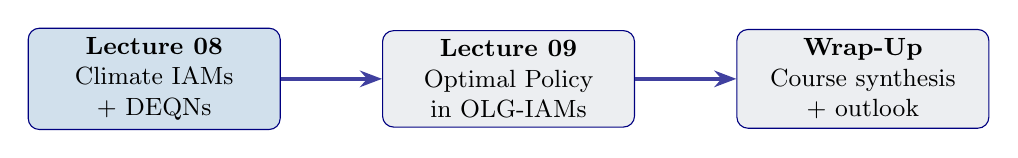
\begin{tikzpicture}[
    box/.style={rectangle, draw=uzhblue, fill=uzhgreylight, rounded corners=4pt,
                minimum width=3.2cm, minimum height=1.1cm, align=center, font=\small},
    arr/.style={-{Stealth[length=2.8mm]}, very thick, uzhblue!75}
]
\node[box, fill=softblue!25] (l08) at (0,0) {\textbf{Lecture 08}\\Climate IAMs\\+ DEQNs};
\node[box] (l09) at (4.5,0) {\textbf{Lecture 09}\\Optimal Policy\\in OLG-IAMs};
\node[box] (l10) at (9,0) {\textbf{Wrap-Up}\\Course synthesis\\+ outlook};

\draw[arr] (l08) -- (l09);
\draw[arr] (l09) -- (l10);
\end{tikzpicture}
\end{center}

\vspace{0.3cm}
\textbf{This lecture}:
\begin{enumerate}
    \item Motivation: why climate economics?
    \item The DICE/CDICE climate model
    \item A stochastic IAM: full model and derivation
    \item Deep uncertainty quantification
\end{enumerate}
\end{frame}

% ============================================================================
% SECTION I: MOTIVATION
% ============================================================================
\section{Motivation --- Why Climate Economics?}

% --- Frame 3: Section Divider ---
\begin{frame}{}
\vfill
\begin{center}
{\Huge \textcolor{uzhblue}{\textbf{Part I}}}\\[12pt]
{\LARGE Why Climate Economics?}
\end{center}
\vfill
\end{frame}

% --- Frame 4: Climate change as economic threat ---
\begin{frame}{Climate Change as an Economic Threat}
\begin{columns}[T]
\column{0.48\textwidth}
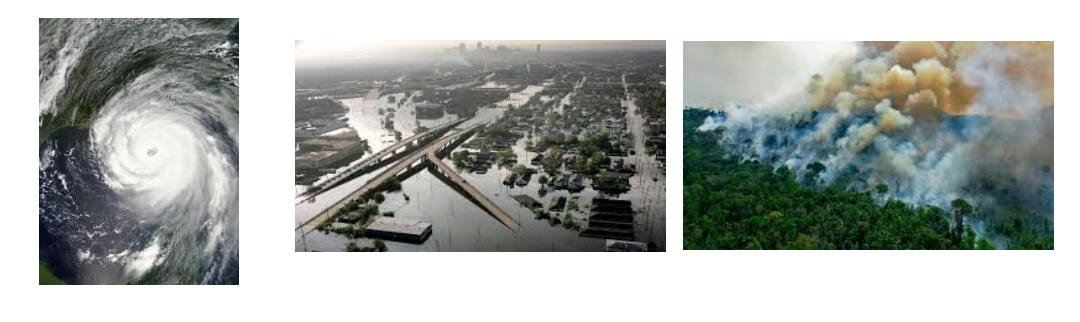
\includegraphics[width=\linewidth]{global-warming.png}
{\footnotesize Observed global warming motivates the IAM feedback loop below.}

\column{0.50\textwidth}
\begin{itemize}
    \item Global warming is a growing threat to economic well-being.
    \item Tipping points place us in catastrophic danger.
    \item Impacts current and future generations in different regions very differently.
    \item Recent overviews: Dietz (2024), van der Ploeg and Rezai (2026), Fernandez-Villaverde, Gillingham, Scheidegger (2025).
\end{itemize}
\end{columns}
\end{frame}

% --- Frame 5: Why IAMs ---
\begin{frame}{Why Integrated Assessment Models (IAMs)?}
\begin{block}{IAM logic}
Couple the \emphc{economy} (output, investment, abatement, welfare) with the \emphc{climate system}
(carbon concentrations, temperature, damages).
\end{block}

\vspace{0.05cm}
\begin{center}
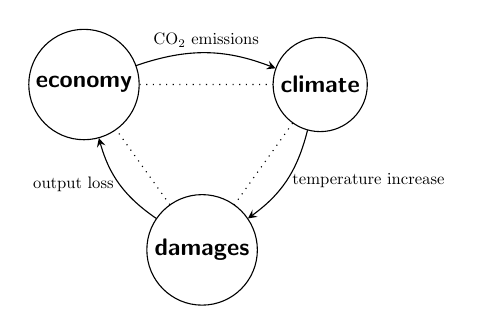
\begin{tikzpicture}[>=stealth, node distance=2cm, scale=0.60, transform shape]
    \tikzstyle{main node} = [circle, draw, minimum size=1.2cm, font=\sffamily\Large\bfseries]
    \node[main node] (economy) at (0,0) {economy};
    \node[main node] (climate) at (5,0) {climate};
    \node[main node] (damages) at (2.5,-3.5) {damages};
    \draw[->] (economy) to[bend left=20] node[above] {CO$_2$ emissions} (climate);
    \draw[->] (climate) to[bend left=20] node[right] {temperature increase} (damages);
    \draw[->] (damages) to[bend left=20] node[left] {output loss} (economy);
    \draw[dotted] (economy) -- (climate) -- (damages) -- (economy);
\end{tikzpicture}
\end{center}

\textbf{Output of interest:} social cost of carbon (SCC), optimal tax paths, welfare decomposition.
\vspace{-0.05cm}
\end{frame}

% --- Frame 6: Social cost of carbon ---
\begin{frame}{The Social Cost of Carbon (SCC)}
\begin{block}{Definition}
SCC at time $t$: marginal welfare cost of one extra unit of emissions, converted to consumption units.
\end{block}

\vspace{0.2cm}
\[
\mathrm{SCC}_t = -\frac{\partial V_t / \partial E_t}{\partial V_t / \partial C_t}
\]

\begin{columns}[T]
\column{0.49\textwidth}
\textbf{High SCC when}
\begin{itemize}
    \item Damages are steep
    \item Climate response is strong
    \item Discounting is low
    \item Tipping risk is material
\end{itemize}

\column{0.49\textwidth}
\textbf{Policy interpretation}
\begin{itemize}
    \item Tax path for carbon pricing
    \item Benchmark for regulation / cap-and-trade
    \item Input to cost-benefit analysis
    \item Why uncertainty matters: SCC is a \emphc{distribution}
\end{itemize}
\end{columns}
\end{frame}

% --- Frame 7: Why computationally hard ---
\begin{frame}{Why This Is Computationally Hard}
\begin{columns}[T]
\column{0.55\textwidth}
\begin{itemize}
    \item \textbf{Nonstationarity}: TFP, population, emissions intensity, and forcing paths all change exogenously over time.
    \item \textbf{Coupled dynamics}: economy and climate interact in both directions.
    \item \textbf{Long horizon}: welfare effects unfold over 100--300 years.
    \item \textbf{Curse of dimensionality}: nonlinearities, tipping hazards, constraints.
\end{itemize}

\column{0.42\textwidth}
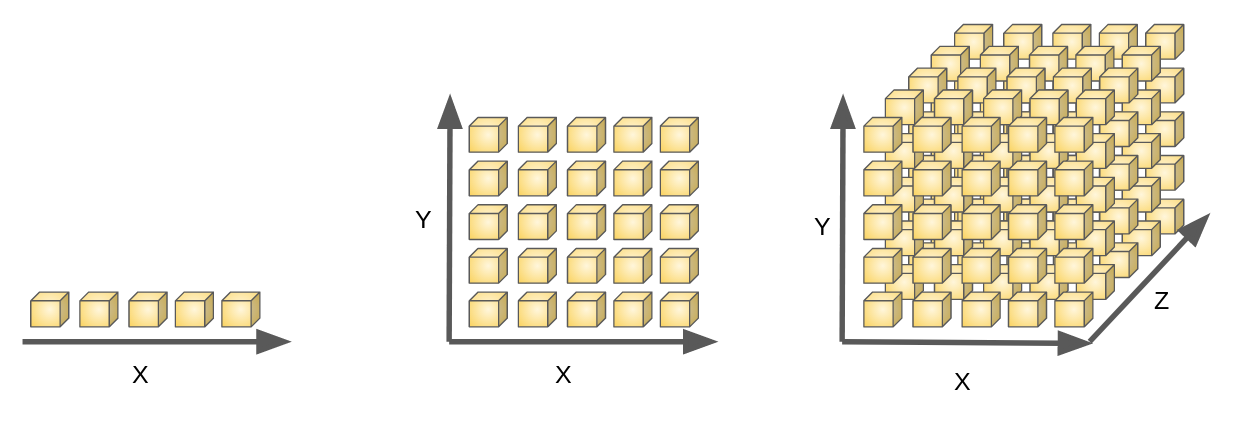
\includegraphics[width=0.88\linewidth]{cod.png}\\[4pt]
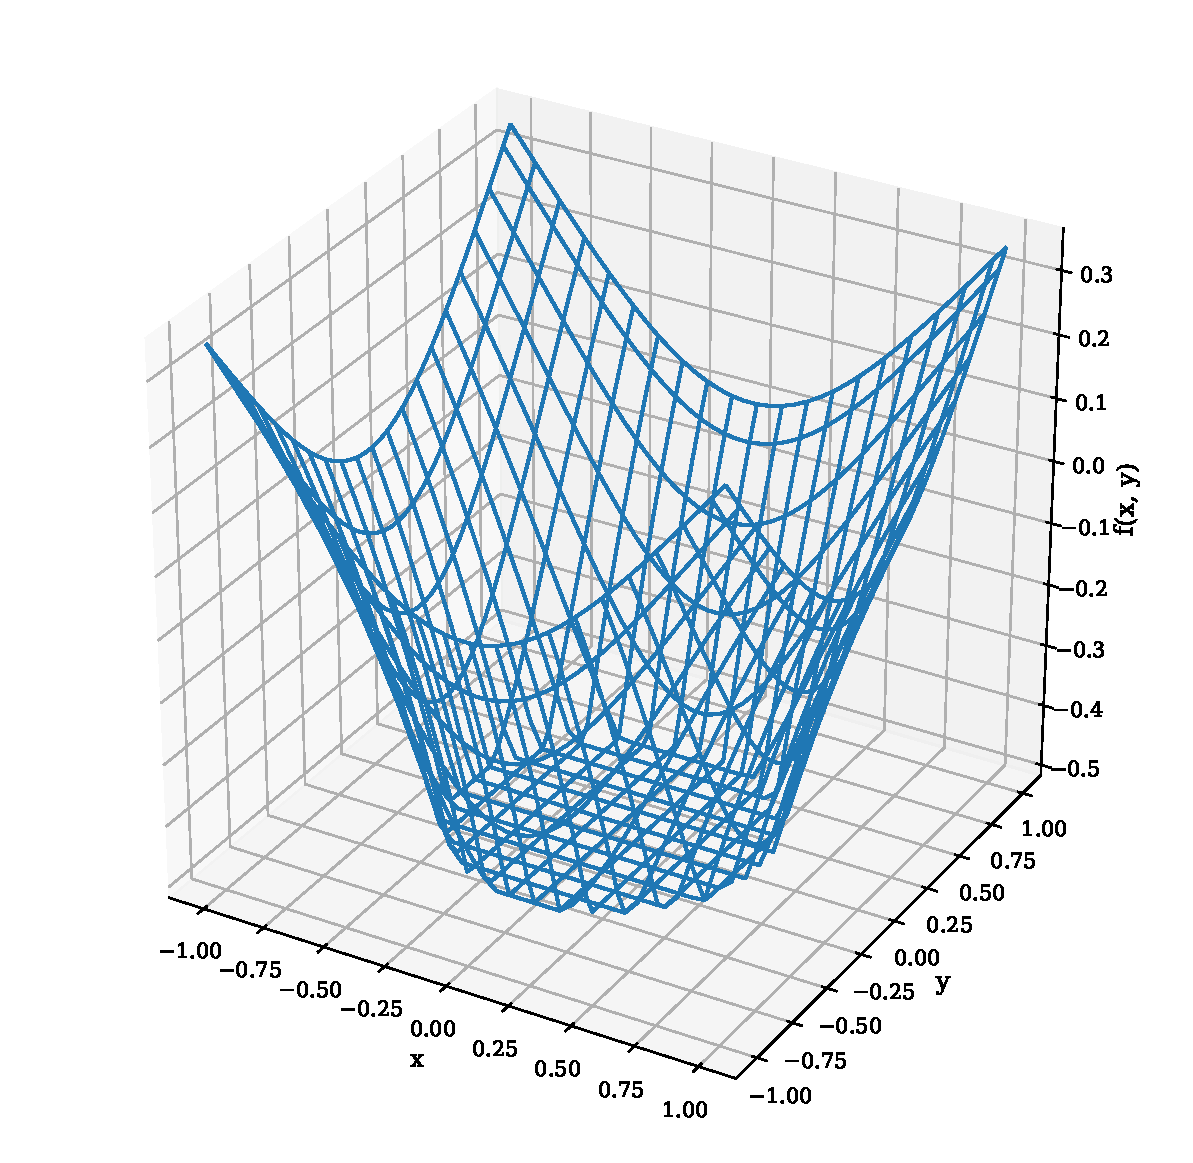
\includegraphics[width=0.88\linewidth]{examplefunc.pdf}
\end{columns}
\end{frame}

% --- Frame 8: Our contribution ---
\begin{frame}{Our Contribution}
\begin{itemize}
    \item \textcolor{blue}{\textbf{Generic global solution method}} to efficiently compute global solutions to stochastic IAMs that include economic and climate risks.
    \item \textcolor{blue}{\textbf{Perform global sensitivity analysis}} with respect to uncertain parameters most discussed in the literature.
\end{itemize}

\vspace{0.2cm}
\begin{enumerate}
    \item Exploit \textbf{deep equilibrium nets} (DEQNs) to alleviate the curse of dimensionality.
    \item Add model parameters as \textbf{pseudo-states} $\rightarrow$ solve the model only \emphc{once}.
    \item Construct \textbf{surrogate models} for the SCC (and other QoIs) using \textbf{Gaussian Process regression} and \textbf{Bayesian active learning}.
\end{enumerate}
\end{frame}

% ============================================================================
% SECTION II: DICE/CDICE CLIMATE MODEL
% ============================================================================
\section{The DICE/CDICE Climate Model}

% --- Frame 9: Section Divider ---
\begin{frame}{}
\vfill
\begin{center}
{\Huge \textcolor{uzhblue}{\textbf{Part II}}}\\[12pt]
{\LARGE The DICE/CDICE Climate Model}
\end{center}
\vfill
\end{frame}

% --- Frame 10: DICE baseline ---
\begin{frame}{DICE Baseline: Minimal Global IAM}
\small
\begin{columns}[T]
\column{0.56\textwidth}
\textbf{State variables}
\begin{itemize}
    \item Economic stock: $K_t$
    \item Carbon stocks: $M_t^{\mathrm{AT}}, M_t^{\mathrm{UO}}, M_t^{\mathrm{LO}}$
    \item Temperature states: $T_t^{\mathrm{AT}}, T_t^{\mathrm{OC}}$
    \item Exogenous trends: population $L_t$, TFP $A_t$, emissions intensity $\sigma_t$
\end{itemize}

\textbf{Controls}
\begin{itemize}
    \item Savings / investment share $s_t$
    \item Abatement rate $\mu_t$
\end{itemize}

\column{0.41\textwidth}
\begin{exampleblock}{Why DICE is influential}
\begin{itemize}
    \item Transparent
    \item Fast to evaluate
    \item Policy-facing
    \item Benchmark for extensions
\end{itemize}
\end{exampleblock}
\end{columns}

\vspace{0.2cm}
\begin{alertblock}{Challenge}
Fast is useful, but only if the climate module is calibrated consistently with climate science.
\end{alertblock}
\end{frame}

% --- Frame 11: Carbon cycle ---
\begin{frame}{Carbon Cycle (3-Box Model)}
\small
\begin{itemize}
    \item DICE-2016 models the carbon cycle via three carbon reservoirs:
    \begin{itemize}
        \item Atmosphere (AT), Upper ocean (UO), Lower ocean (LO)
    \end{itemize}
    \item Aggregate distribution of carbon: $M_t = (M_{\mathrm{AT},t}, M_{\mathrm{UO},t}, M_{\mathrm{LO},t})^T$
\end{itemize}

\vspace{0.2cm}
\textbf{Carbon concentrations evolve as a linear dynamic system:}
\[
M_{t+1} = (I + \Delta_t \cdot B) \cdot M_t + \Delta_t \cdot E_t
\]

\begin{itemize}
    \item Carbon emissions (economic activity + exogenous source): $E_t = E_{\mathrm{ind},t} + E_{\mathrm{Land}}$
    \item Industrial emissions: $E_{\mathrm{ind},t} = (1-\mu_t)\sigma_t K_t^{\alpha}(A_t L_t)^{1-\alpha}$
    \item $B$ is the transfer matrix governing exchange rates between reservoirs
\end{itemize}
\end{frame}

% --- Finger Exercise: Carbon Cycle ---
\begin{frame}{\exercisepause{} Finger Exercise: One-Step Carbon Cycle}
\begin{exampleblock}{Exercise}
The simplified carbon cycle has atmospheric CO$_2$ evolving as:
\[
M_{\text{AT}}^{t+1} = E_t + \phi_{11}\, M_{\text{AT}}^{t} + \phi_{21}\, M_{\text{UP}}^{t},
\]
where $\phi_{11} = 0.912$, $\phi_{21} = 0.0444$, and $M_{\text{UP}}^t$ (upper ocean) is given.
\begin{enumerate}
    \item With $M_{\text{AT}}^{2020} = 851$ GtC, $M_{\text{UP}}^{2020} = 628$ GtC, and emissions $E_{2020} = 10$ GtC/yr (over a 5-year step: $E = 50$ GtC): compute $M_{\text{AT}}^{2025}$.
    \item If emissions doubled to $E = 100$ GtC, what would $M_{\text{AT}}^{2025}$ be?
    \item By how many GtC does doubling emissions increase atmospheric CO$_2$?
\end{enumerate}
\end{exampleblock}
\end{frame}

\begin{frame}{Solution: One-Step Carbon Cycle}
\begin{block}{Answer}
\begin{enumerate}
    \item $M_{\text{AT}}^{2025} = 50 + 0.912 \times 851 + 0.0444 \times 628 = 50 + 776.1 + 27.9 = 854.0$ GtC.
    \item $M_{\text{AT}}^{2025} = 100 + 776.1 + 27.9 = 904.0$ GtC.
    \item Doubling emissions adds $904.0 - 854.0 = 50$ GtC---exactly the extra emissions.  The carbon cycle is \emphc{linear} in emissions (at one-step horizon), so the effect is additive.
\end{enumerate}
\end{block}
\end{frame}

% --- Frame 12: Temperature dynamics ---
\begin{frame}{Temperature Dynamics (2-Box Model)}
\small
The two-layer energy balance model in DICE-2016:
\begin{align*}
    T^{\mathrm{AT}}_{t+1} &= T^{\mathrm{AT}}_{t} + \Delta_t \cdot c_{1} \left(F_{t} - \lambda T^{\mathrm{AT}}_{t} - c_{3}\left(T^{\mathrm{AT}}_{t} - T^{\mathrm{OC}}_{t}\right)\right) \\
    T^{\mathrm{OC}}_{t+1} &= T^{\mathrm{OC}}_{t} + \Delta_t \cdot c_{4} \left(T^{\mathrm{AT}}_{t} - T^{\mathrm{OC}}_{t}\right)
\end{align*}

\textbf{Radiative forcing:}
\[
    F_{t} = F_{\mathrm{2\times CO_2}} \frac{\log(M^{\mathrm{AT}}_{t}/M^{\mathrm{AT}}_{\mathrm{EQ}})}{\log(2)} + F^{\mathrm{EX}}_{t}
\]

\begin{alertblock}{Key parameters}
$\lambda = F_{\mathrm{2\times CO_2}}/\Delta T_{\mathrm{AT},\times 2}$ where $\Delta T_{\mathrm{AT},\times 2}$ is the \emphc{equilibrium climate sensitivity} (ECS) --- the long-run warming from CO$_2$ doubling.
\end{alertblock}
\end{frame}

% --- Frame 13: Damage functions ---
\begin{frame}{Damage Functions}
\footnotesize
\begin{columns}[T]
\column{0.38\textwidth}
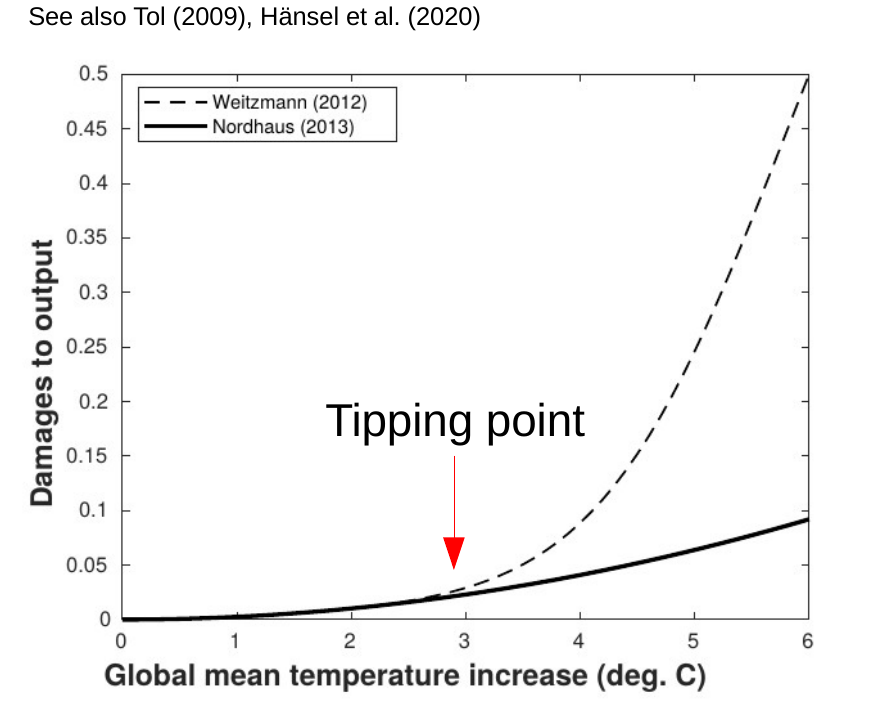
\includegraphics[width=0.88\linewidth]{damge.png}
{\scriptsize Retained-output damage factors decline as warming rises.}

\column{0.60\textwidth}
\textbf{Nordhaus (2013):}
\[
\Omega^N_t(T_{\mathrm{AT},t}) = \frac{1}{1 + \pi_1 T_{\mathrm{AT},t} + \pi_2 T_{\mathrm{AT},t}^2}
\]

\textbf{Weitzman (2012) --- with tipping:}
\[
\Omega_t(T_{\mathrm{AT},t}) = \frac{1}{1 + \left(\frac{1}{\psi_1} T_{\mathrm{AT},t}\right)^{2} + \left(\frac{1}{2 \cdot TP_t} T_{\mathrm{AT},t}\right)^{6.754}}
\]
\end{columns}

\vspace{0.2cm}
\begin{itemize}
    \item Degree of convexity is of key importance in determining the optimal taxes [Weitzman 2012].
    \item Tipping points: losing the Amazon rain forest, faster onset of El Ni\~no, reversal of the Gulf Stream, etc.
\end{itemize}
\end{frame}

% --- Frame 14: Why recalibrate ---
\begin{frame}{Why Recalibrate? $\rightarrow$ CDICE}
\small
\begin{itemize}
    \item Climate emulators must reproduce benchmark behavior from climate science model archives (CMIP).
    \item Earlier critiques (Dietz et al., 2021) highlighted major discrepancies for common IAM calibrations.
    \item Folini et al.\ show that the \emphc{functional form can remain simple}, but parameters require systematic calibration.
\end{itemize}

\vspace{0.2cm}
\begin{center}
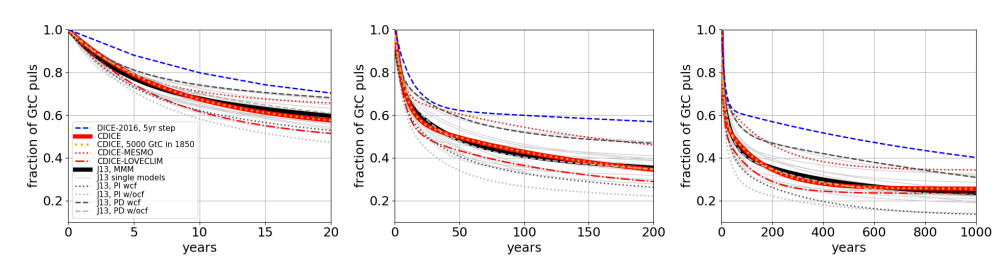
\includegraphics[width=0.88\textwidth]{CDICE-vs-DICE.png}
\end{center}
{\footnotesize CDICE recalibrates the reduced-form climate emulator to climate-science benchmarks.}
\end{frame}

% --- Frame 15: Four-test framework ---
\begin{frame}{Four-Test Framework (Folini et al., 2024)}
\scriptsize
\begin{center}
\begin{tabular}{lll}
\toprule
\textbf{Test} & \textbf{Targets} & \textbf{Use} \\
\midrule
1. Carbon pulse (100 GtC) & Atmospheric retention path & Calibrate carbon cycle \\
2. 4$\times$CO$_2$ step & Temperature impulse response & Calibrate temperature block \\
3. 1\% CO$_2$/year & Transient climate response (TCR) & Out-of-sample validation \\
4. Historical + RCP & Realistic forcing paths & End-to-end validation \\
\bottomrule
\end{tabular}
\end{center}

\vspace{0.2cm}
\begin{columns}[T]
\column{0.48\textwidth}
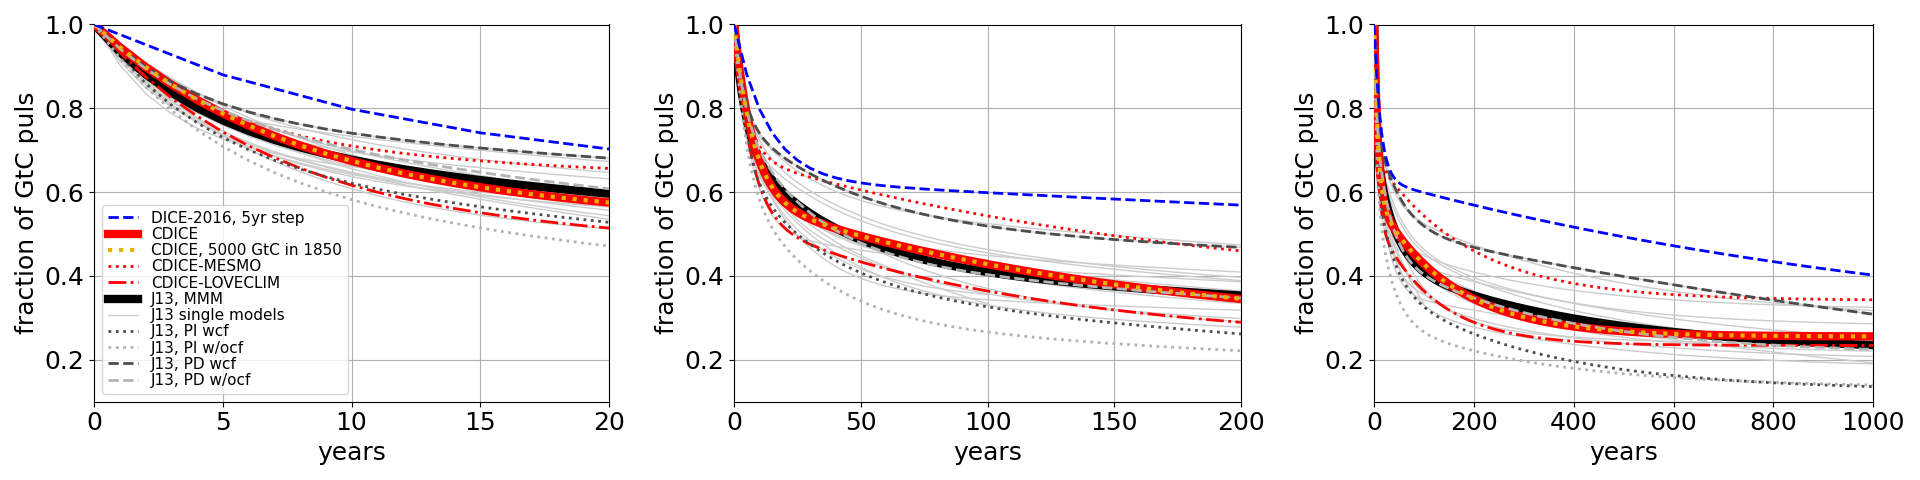
\includegraphics[width=\linewidth]{CCBM_100GtC_Puls.png}
{\footnotesize Carbon-pulse response.}

\column{0.48\textwidth}
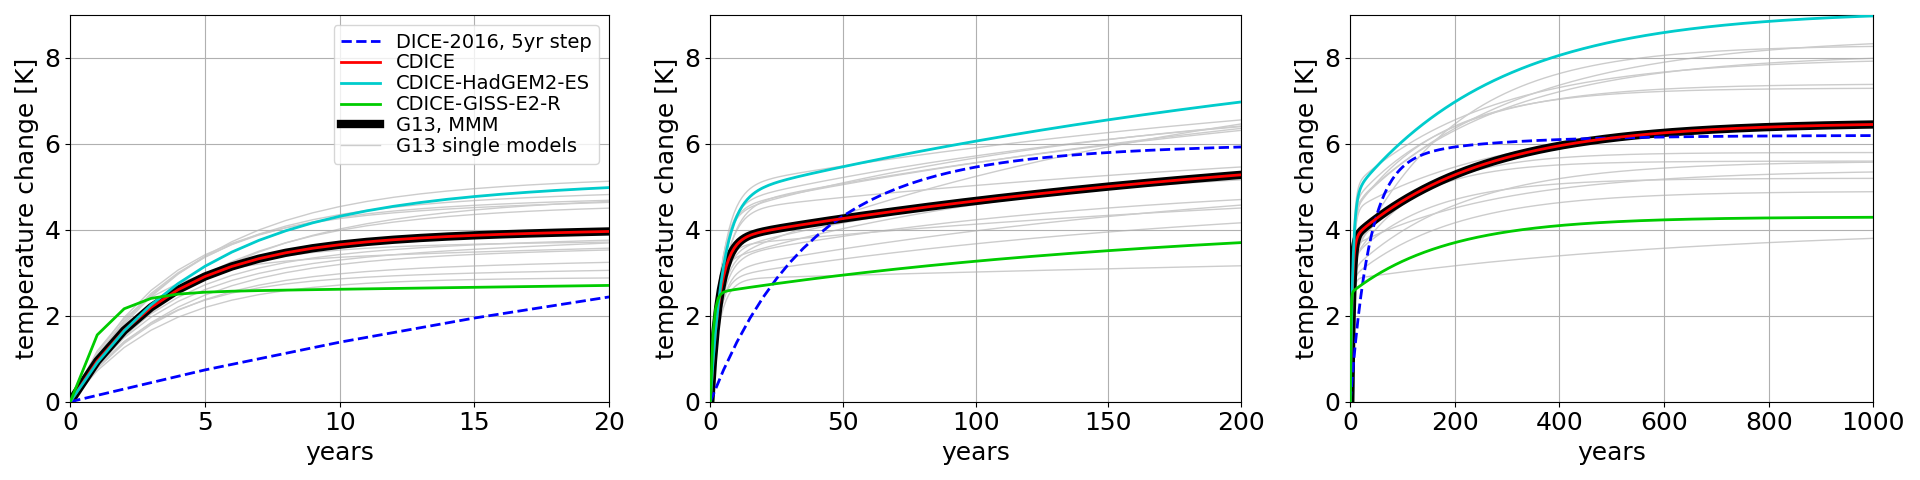
\includegraphics[width=\linewidth]{TempBM_4xCO2_on_PI.png}
{\footnotesize Temperature response to a $4\times$CO$_2$ forcing step.}
\end{columns}
\end{frame}

% --- Frame 16: ECS uncertainty ---
\begin{frame}{Equilibrium Climate Sensitivity (ECS) --- A Key Uncertainty}
\begin{center}
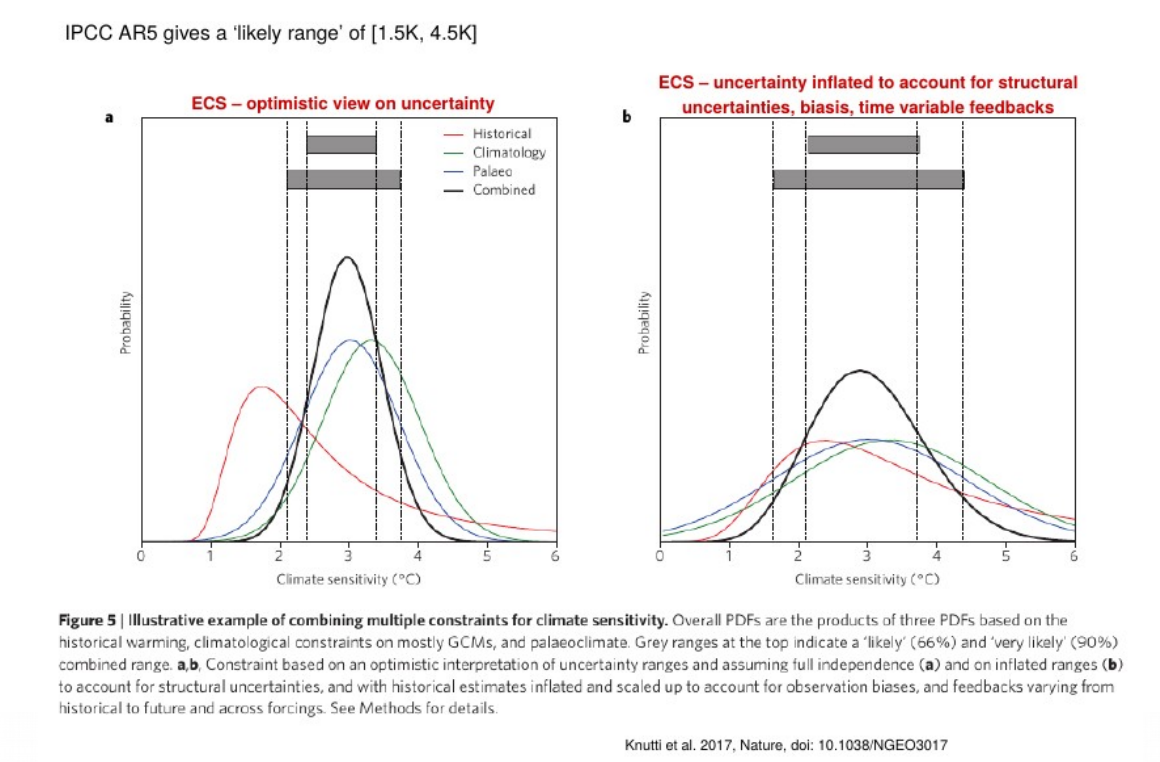
\includegraphics[width=0.50\textwidth]{knutti.png}
\end{center}

\vspace{-0.15cm}
\small
\begin{itemize}\setlength\itemsep{0pt}
    \item Roe and Baker (2007): $\mathrm{ECS} = \frac{\lambda_0}{1-f} F_{\mathrm{2\times CO_2}}$, $f \sim \mathcal{N}(\mu_f, S_f)$.
    \item Making ECS stochastic is a natural channel for Bayesian learning.
\end{itemize}
\end{frame}

% --- Frame 17: Transparent time step ---
\begin{frame}{Transparent Time-Step Formulation}
\small
A practical contribution in CDICE: expose the time-step scaling directly in equations.
\[
X_{t+\Delta t} = X_t + \Delta t \cdot f(X_t, u_t; \theta)
\]

\begin{itemize}
    \item Allows coherent annual, 5-year, or 10-year implementations within one generic formulation.
    \item Time discretization consistency improves transferability between classroom code, production code, and policy simulation horizons.
\end{itemize}

\vspace{0.2cm}
\textbf{Summary of climate module:}
\begin{center}
\small
\begin{tabular}{ll}
\toprule
\textbf{Climate states (5)} & $M_{\mathrm{AT}}, M_{\mathrm{UO}}, M_{\mathrm{LO}}, T^{\mathrm{AT}}, T^{\mathrm{OC}}$ \\
\textbf{Key parameters} & ECS ($\Delta T_{\mathrm{AT},\times 2}$), carbon transfer $B$, forcing $F_{\mathrm{2\times CO_2}}$ \\
\textbf{Uncertainty channels} & ECS, damage curvature, tipping \\
\bottomrule
\end{tabular}
\end{center}
\end{frame}

% ============================================================================
% SECTION III: STOCHASTIC IAM --- FULL MODEL & DERIVATION
% ============================================================================

\end{document}
